\chapter{Ray Tracing}
\label{chap:ray-tracing}

In the previous chapter, track generation was discussed. Once the tracks are laid across the geometry, they need to be partitioned by source region intersections into segments across which the \ac{MOC} equations can be applied. At a minimum, the segment lengths and associated source region identifiers need to be recorded for each track. During the transport sweep, the \ac{MOC} equations described in Chapter~\ref{chap:moc} are applied to all segments. This chapter discusses ray tracing procedures in which the segments are formed from the track and geometry information. Section~\ref{sec:rt-intro} provides an introduction of common ray tracing schemes and their implications. In Section~\ref{hi}.

FIXME

MENTION 2D/1D distinction

\section{Introduction to Ray Tracing}
\label{sec:rt-intro}

Ray tracing fundamentally solves the problem of determining the next intersection with a surface along a direction of travel and which new region is entered after the intersection. Since complicated geometries contain many surfaces, this can be expensive if all surfaces in the geometry need to be tested for intersections. Much of the work in complex ray tracing for animations relies on somehow forming \textit{acceleration structures} which limit the number of surfaces that need to be tested~\cite{acceleration-structures}. Traditional methods form acceleration structures that resemble some hierarchy of cells and surfaces grouped by location so that only nearby surfaces are considered~\cite{acc-struct-hierarchy}.

In traditional reactor physics problems, an acceleration structure is naturally formed by the hierarchical structure of the geometry. For instance, a core can largely be viewed as an arrangement of assemblies, each of which is comprised of an arrangement of fuel rods. Therefore, by just using the hierarchical \ac{CSG} form of the geometry, the ray tracing requirements are naturally reduced.

However, ray tracing can still be expensive, especially for cases which do not form an easily structured form, such as reactor baffles, grid spacers, and neutron shields. These complexities cause a generic algorithm capable of treating all the reactor detail to lose computational efficiency. In moving from 2D simulations to 3D simulations, even more surfaces are introduced, exacerbating the issue.
	
Most \ac{MOC} implementations avoid this issue by treating ray tracing as a pre-processing step whereby the segment information, which includes its length and the ID of the traversed \ac{SR}, is calculated and explicitly stored at the beginning of the simulation and then loaded during the transport sweep. In this way  the amount of repeated ray tracing work is reduced and the cost of ray tracing is effectively amortized over the number of transport sweeps. While this approach is straightforward, its memory and compute requirements for 3D \ac{MOC} can be prohibitive, even for small problems, due to the vast number of segments present in 3D \ac{MOC} simulations~\cite{physor2016otf}. Reducing the memory footprint is important for many reasons including improved cache efficiency and reducing bulk memory requirements.

In this thesis, an alternative approach is presented that greatly reduces the segment storage and generation requirements by taking advantage of the extruded geometry structure common to many reactor physics problems. This alternative approach saves no 3D segment data, rather treating the ray tracing problem as a coupled 2D and 1D system whereby 2D radial ray tracing information is combined with 1D axial information to compute the 3D intersections~\cite{pyhsor2016otf}.

Another ray tracing scheme, termed the \ac{CCM}~\cite{Sciannandrone2015}, also sought to reduce the memory requirements for ray tracing axially extruded geometries by only saving the unique chords (or segments).  However, this method still requires that the segmentation procedure be performed for all 3D tracks prior to performing transport sweeps, which can be prohibitively expensive for complex geometries. In addition, while it does indeed reduce the storage requirements, the storage scales with the number of unique 3D segment lengths. This can be problematical for problems in which there are a large number of unique segments. For large full core problems, some regions might indeed have many repeated segment lengths, but regions for which the source height is similar to the axial ray spacing, there would be very few repeated segment lengths.

The implementation in this thesis aims to most efficiently solve typical \ac{PWR} problems. From experience in simulating single \ac{PWR} assemblies, the axial ray separation can be on the same order as the axial source height~\cite{openmoc-beavrs}, potentially causing there to be a large number of unique segments. This motivates using concepts from the \ac{CCM} method to identify repeated segment lengths but also relying on the 2D/1D ray tracing approach to reduce storage.

\section{Forming an Axially Extruded Geometry}
\label{sec:ax-extruded}

As previously stated, OpenMOC only supports piece-wise axially extruded geometries. Most common reactor problems are naturally defined as piece-wise axially extruded so this is not a strong limitation in practice. Here, an axially extruded geometry is defined to be a geometry in which every radial slice of the reactor geometry is identical whereas a piece-wise axially extruded geometry can be defined as the collection of a finite number of axial zones where the geometry over each axial zone constitutes an extruded geometry. 

For ray tracing in a 2D/1D scheme, a single axially extruded extruded geometry is required. Therefore, all radial detail must be gathered in order to effectively convert the piece-wise axially extruded geometry to an axially extruded geometry. While common reactor cores contain variations from axially extruded geometries, such as end plugs for control rods, these variations can be fully captured at little cost by implicitly inserting additional geometric intersections. 

Note the axially extruded requirement is only applied to the geometry, not the materials. Each axially extruded region could be comprised of various materials. Given an axially extruded geometry, it is possible to store only the 2D segments associated with intersections in the radial geometry. The 3D segments can then be formed on-the-fly using a simple axial mesh.

First, 2D segments need to be formed which reflect intersections of the 2D tracks with a superposition of all radial surfaces in the geometry. This is done by simultaneously ray tracing across all the unique radial planes in the geometry, as depicted in Fig.~\ref{fig:superposition}. This creates an implicit geometry containing all radial information, termed the \textit{superposition plane}. The 2D geometric regions in the superposition plane correspond to an axially extruded region with an associated unique identifier that contains an axial mesh and an array of associated 3D \ac{SR}s. 

\begin{figure}[ht!]
	\centering
	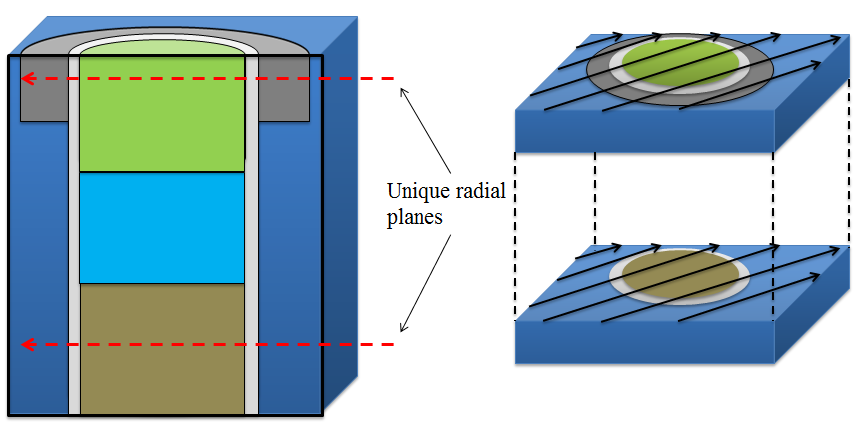
\includegraphics[width=\linewidth]{figures/ph2016/new_unique_z_levels_v_extruded_rt2.png}
	\caption{Depiction of 2D ray tracing for superposition of all radial detail.}
	\label{fig:superposition}
\end{figure}

Each 2D segment formed during the ray tracing contains its length and the unique identifier of the axially extruded region being traversed. After 2D segmentation, axial meshes need to be created for on-the-fly axial ray tracing. If a global axial mesh is desired, whereby all axially extruded regions have the same axial mesh, all the unique z-planes in the geometry are collected and sorted into a single axial mesh. Otherwise, local meshes are populated for each axially extruded region during initialization of the 3D \ac{SR}s. To initialize the 3D \ac{SR}s, a temporary vertical ray is created for each axially extruded region. These rays are all upward directed, starting from the bottom of the root geometry, and segmented to determine distances between axial intersections while initializing the associated \ac{SR}s. During this step, the location of a point within each \ac{SR} is noted, and the data structures associated with managing the \ac{SR}s are initialized. An illustration of this process is presented in Fig.~\ref{fig:fsr-initialization}.

\begin{figure}[h!]
	\centering
	\begin{subfigure}[b]{0.25\textwidth}
		\centering
		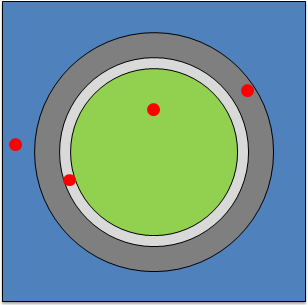
\includegraphics[width=\linewidth]{figures/ph2016/fsr-init-a.PNG}
		\caption{}
		\label{fig:fsr-init-a}
	\end{subfigure}
	\begin{subfigure}[b]{0.28\textwidth}
		\centering
		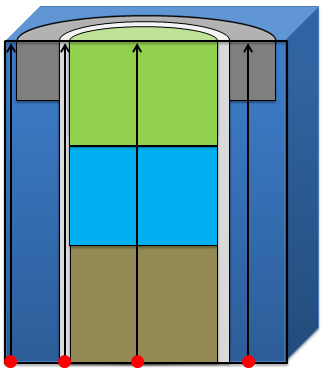
\includegraphics[width=\linewidth]{figures/ph2016/fsr-init-b.PNG}
		\caption{}
		\label{fig:fsr-init-b}
	\end{subfigure}
	\begin{subfigure}[b]{0.4\textwidth}
		\centering
		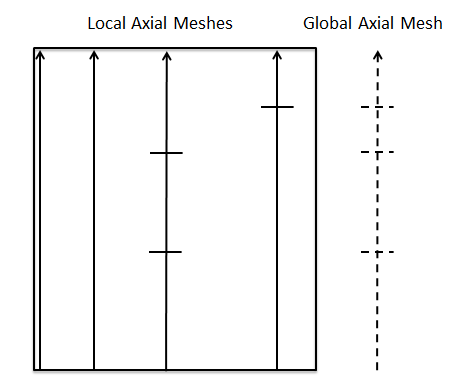
\includegraphics[width=\linewidth]{figures/ph2016/fsr-init-c.PNG}
		\caption{}
		\label{fig:fsr-init-c}
	\end{subfigure}
	\caption[]{Illustration of \ac{SR} initialization starting from the superposition plane (a) where a radial point is chosen in each unique region, vertical tracks (b) are generated at the chosen points to map the axial detail, yielding (c) the 1D axial meshes for each region, and (optionally) a global 1D axial mesh}
	\label{fig:fsr-initialization}
\end{figure}

Implicitly, this strategy can create extra radial intersections since some of the axial levels might not have originally contained the full radial detail of the superposition plane. However, the number of additional intersections should be low due to the regular structure of most reactor cores. For instance, fuel rods with end plugs present only a slight deviation from an axially extruded geometry.

The advantage of local axial meshes is the ability to have different axial refinements within the reactor. For instance, a partially inserted control rod might need a finer \ac{SR} discretizations near the control rod tip. If a global axial mesh were used, the finer discretization would need to be applied to the whole core at that axial height, including the reflector. With local axial meshes, only the regions which need refinement would use a finer discretization.

\section{On-the-fly Axial Ray Tracing}

During the transport sweeps, all 3D tracks are traversed across their span of the geometry. The common method mentioned in Section~\ref{sec:rt-intro}, in which segments are formed in a pre-processing step, accomplishes this by splitting every 3D track into 3D segments before the transport sweeps and then simply cycling through all the segments.

In the methods presented here, 3D segments are recreated on-the-fly using information from the 2D ray trace over all radial detail and the 1D axial meshes, both formed at the beginning of the simulation. Due to the manner in which the 3D tracks were generated, as detailed in Chapter~\ref{chap:track-laydown}, each 3D track has a corresponding 2D segmented track. From the starting $z$ coordinate of a track along with its polar angle, it is possible to determine the distance along the track to both intersections with axial planes and intersections with 2D surfaces, defined by the 2D segments. On-the-fly axial ray tracing can either be performed on each 3D track individually or on an entire $z$-stack.

\subsection{Ray Tracing Individual 3D Tracks}

For ray tracing each 3D track individually, the associated 2D segments are traversed until the 3D track reaches its endpoint. First, the starting point is used to determine the appropriate starting 2D segment and index into the axial mesh. If local axial meshes are used, the index needs to be recomputed with a binary search at the start of each 2D segment. If a global mesh is used, the axial index only needs to be calculated at the beginning of the track. The 2D segments are traversed and the shorter distance to either an axial or radial intersection is calculated. This computed distance is the 3D segment length and has an associated 3D \ac{SR} indicated by the axial index. To form the next 3D segment, the position along the 2D track is moved by the appropriate distance. This process is repeated until the endpoint is reached. An illustration of this concept is presented in Fig.~\ref{fig::otf_ray_tracing}.

\begin{figure}[ht!]
	\centering
	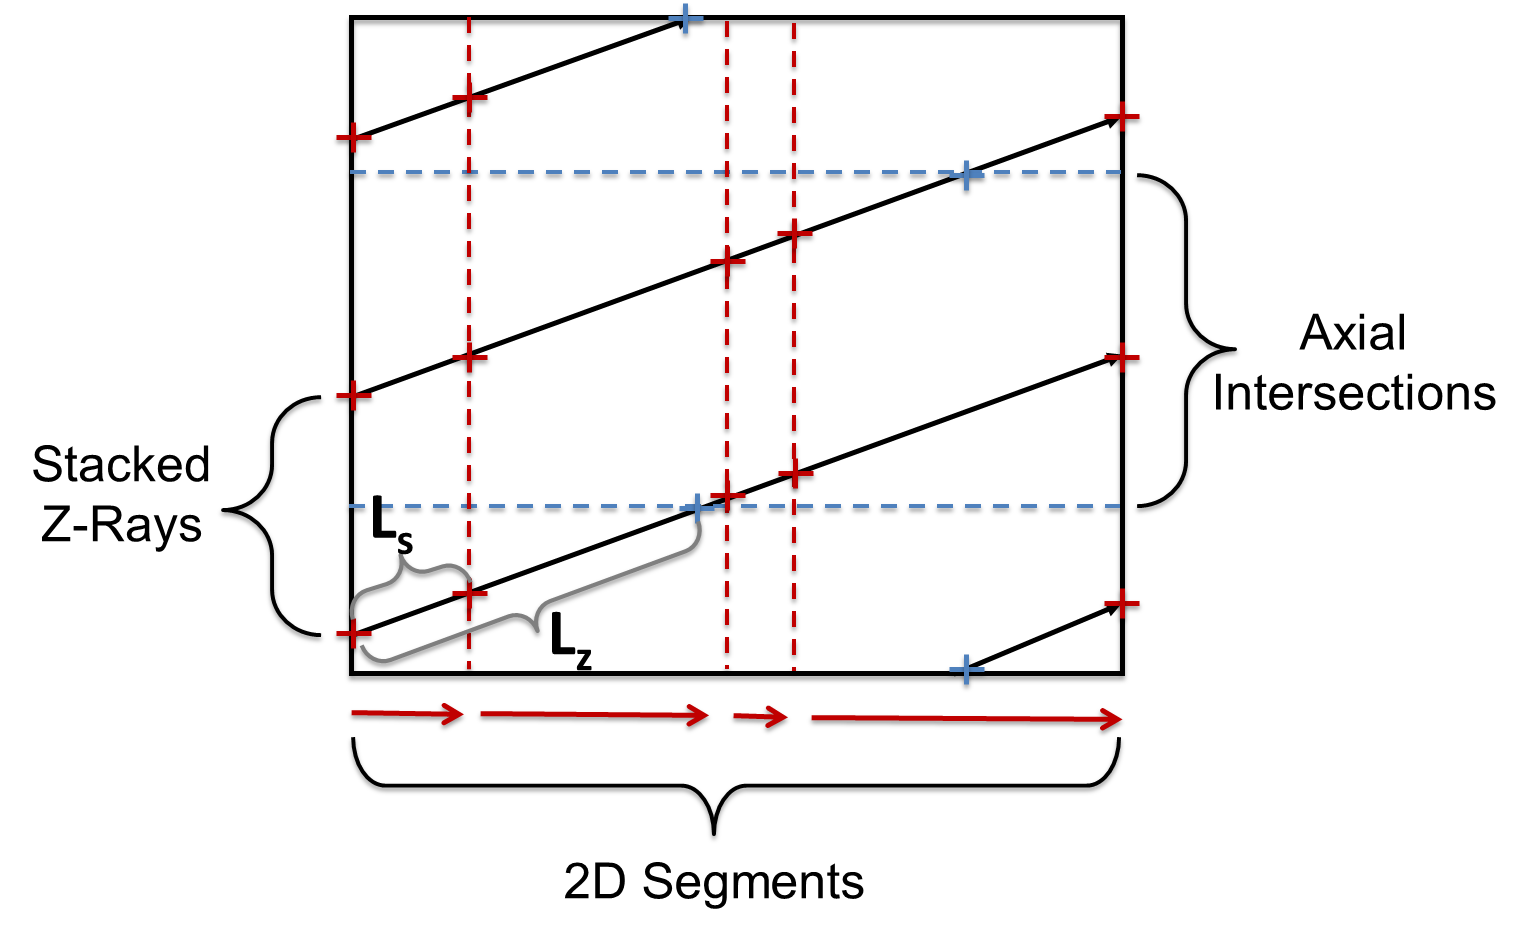
\includegraphics[width=0.75\linewidth]{figures/ph2016/otf_ray_tracing.png}
	\caption{Illustration of the on-the-fly axial ray tracing process with axial intersections colored in blue and radial intersections colored in red. For the chosen track, the distance to the next axial intersection is denoted $L_z$ and the the distance to the next radial intersection is denoted $L_s$.}
	\label{fig::otf_ray_tracing}
\end{figure}

\subsection{Ray Tracing 3D Track $z$-Stacks}

The structure of the 3D track laydown can be used to ray trace an entire $z$-stack. Specifically all tracks in the $z$-stack have the same polar angle $\theta$, project onto the same 2D track, and are separated by a constant axial ray spacing $\delta z$. Therefore, the axial height $z_i$ of the $i^{\textit{th}}$ lowest track (starting from 0) can be given as a function of distance $s$ along the associated 2D track as
\begin{equation}
z_i(s) = z_0(0) + i\delta z + s \cot{\theta}
\label{eq::track_projection}
\end{equation}
where $z_0(0)$ is the $z$-coordinate at the intersection of the lowest track with the $z$-axis at the start of the associated 2D track. Combining this with 2D track information is enough to completely describe the trajectory and location of 3D tracks in the stack. Therefore, it is possible to determine which tracks will traverse a given \ac{SR}.

For each 2D segment in the 2D track, there is an associated axially extruded region which contains a list of 3D \ac{SR}s in the region. To trace a $z$-stack, intersections within axially extruded \ac{SR}s are determined in the order traversed by the 2D segments. The 1D axial mesh (either local or global) associated with the axially extruded region is used to determine the axial boundaries of each 3D \ac{SR}. Using the boundaries of the \ac{SR} and Eq.~\ref{eq::track_projection}, it is possible to analytically compute the indexes of tracks that will cross the \ac{SR} as
\begin{equation}
i_{\textit{start}} = \Bigg\lceil\frac{z_{\textit{min}} - \max\left({z_0(s_{\textit{start}}), z_0(s_{\textit{end}})}\right) }{\delta z}\Bigg\rceil
\label{eq::start_track}
\end{equation}
\begin{equation}
i_{\textit{end}} = \Bigg\lfloor\frac{z_{\textit{max}} - \min\left({z_0(s_{\textit{start}}), z_0(s_{\textit{end}})}\right) }{\delta z}\Bigg\rfloor
\label{eq::end_track}
\end{equation}
where $i_{\textit{start}}$ is the index of the first track to cross the \ac{SR}, $i_{\textit{end}}$ is the index of the last track to cross the \ac{SR}, $s_{\textit{start}}$ is the 2D distance traversed at the start of the segment and $s_{\textit{end}}$ is the 2D distance traversed at the end of the segment. A detailed derivation of these relationships can be found in Appendix~\ref{app:z-stack}. A depiction of this process is shown in Fig.~\ref{fig::stack_tracing}.

\begin{figure}[ht!]
	\centering
	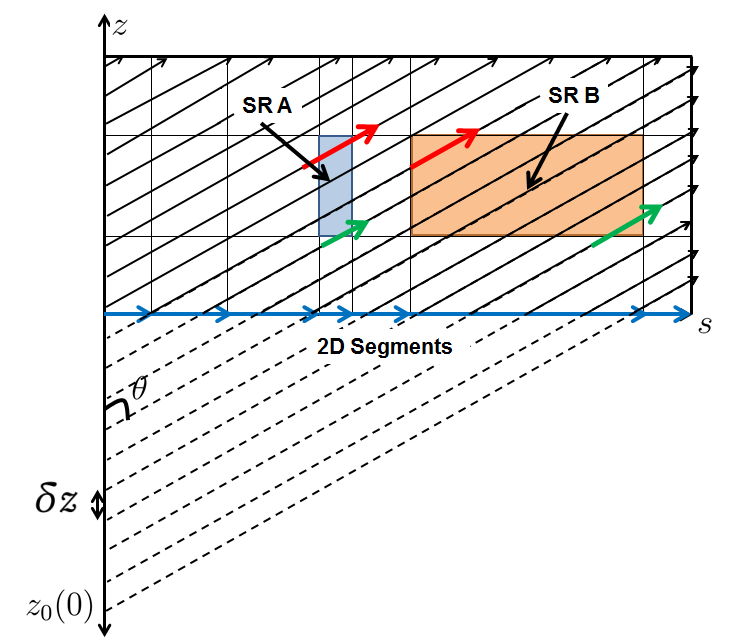
\includegraphics[width=0.75\linewidth]{figures/ph2016/stack_tracing.png}
	\caption{Illustration of the on-the-fly axial ray tracing process for an entire $z$-stack. The green arrows denote the first track to traverse the highlighted \ac{SR}s calculated by Eq.~\ref{eq::start_track} and the red arrows denote the last tracks to traverse the \ac{SR}s calculated by Eq.~\ref{eq::end_track}.}
	\label{fig::stack_tracing}
\end{figure}


Notice that for \ac{SR} A depicted in Fig.~\ref{fig::stack_tracing} there are multiple track segments that cross the entire 2D length of the \ac{SR} and are therefore identical. Their 3D segment length $L_{3D}$ would simply be
\begin{equation}
L_{3D} = \frac{s_{\textit{end}} - s_{\textit{start}}}{\sin{\theta}}.
\end{equation}

In common reactor physics problems we expect this effect to be much more pronounced. Due to the radial direction having much greater complexity than the axial direction, \ac{SR}s will tend to be longer in the axial direction than in the radial plane, especially when higher order sources are added in the axial direction. The high aspect ratio causes some tracks to cross the entire 2D length of the \ac{SR}.

To take advantage of this, it is possible to calculate the indexes of the first and last tracks to traverse the entire 2D segment length. For this condition to be met, the axial height of the tracks over the entire 2D segment must be greater than the minimum axial boundary of the \ac{SR} and less than the maximum axial boundary. Therefore, the indexes of interest are the first track to have its lowest point above the minimum boundary and the first track to have its highest point above the maximum boundary. These indexes, $i_{\textit{in}}$ and $i_{\textit{out}}$, respectively, can be calculated as:

\begin{equation}
i_{\textit{in}} = \Bigg\lceil\frac{z_{\textit{min}} - \min\left({z_0(s_{\textit{start}}), z_0(s_{\textit{end}}})\right) }{\delta z}\Bigg\rceil
\end{equation}

\begin{equation}
i_{\textit{out}} = \Bigg\lceil\frac{z_{\textit{max}} - \max\left({z_0(s_{\textit{start}}), z_0(s_{\textit{end}}})\right) }{\delta z}\Bigg\rceil
\end{equation}

A derivation of these relations an be found in Appendix~\ref{app:z-stack}. For each \ac{SR} these indexes are calculated along with the beginning and end track indexes given in Eq.~\ref{eq::start_track} and Eq.~\ref{eq::end_track}. It is possible that $i_{\textit{in}}$ will be greater than $i_{\textit{out}}$ when the polar angle is steep enough, allowing for the \ac{SR} to be fully traversed axially without traversing the entire 2D length. These tracks can be determined with indexes $i_{\textit{in}}$ and $i_{\textit{out}}$ and have a common 3D segment length $L_{3D}$ given by
\begin{equation}
L_{3D} = \frac{z_{\textit{max}} - z_{\textit{min}}}{\left| \cos{\theta}\right|}.
\end{equation}

Therefore, 3D segments are classified into four categories:

\begin{itemize}
	\item \textbf{Mixed Tracks -- Case A:} Tracks that partially traverse the \ac{SR} and cross the lower \ac{SR} boundary. They are defined by track indexes $i_{\textit{start}} \leq i < \min\left(i_{\textit{in}}, i_{\textit{out}}\right)$. For these tracks, each 3D segment is computed individually. 
	\item \textbf{Mixed Tracks -- Case B:} Tracks that partially traverse the \ac{SR} and cross the upper \ac{SR} boundary and each 3D segment is again computed individually. They are defined by track indexes $\max\left(i_{\textit{in}}, i_{\textit{out}}\right)  \leq i  \leq i_{\textit{end}}$.
	\item \textbf{Horizontal Tracks:} Tracks that fully traverse the entire 2D radial distance of the \ac{SR} and are defined by indexes $i_{\textit{in}} \leq i < i_{\textit{out}}$. 
	\item \textbf{Vertical Tracks:} Tracks that traverse the entire axial distance of the \ac{SR} and are defined by $i_{\textit{out}} \leq i < i_{\textit{in}}$.
\end{itemize}

This classification of segments allows the computational work involved in calculating track intersections to be greatly reduced. In addition, the horizontal and vertical tracks for each \ac{SR} have common segment lengths, allowing for the potential reduction in computational work. While not implemented for this thesis, these common segment lengths all have the same exponential term for the \ac{MOC} equations, allowing these terms to only be computed once for the group of equal length segments.

Another important distinction between this scheme and ray tracing by individual 3D track is the traversal order of segments. Since the ray tracing by $z$-stack scheme describes intersections of all tracks with a given region, segments are traversed by \textit{region} rather than by track. In this scheme, the algorithm loops over all regions which are intersected by the $z$-stack, treating all segments which intersect the region before moving to the next region. This has profound implications on cache performance and is the subject of the next section.

\section{Cache Considerations for Segment Traversal}

%When CPU cores load information from memory, they load entire cache lines into local caches rather than just the desired variable. This allows the number of loads to be reduced if nearby memory is accessed. When desired memory is already within the cache of the CPU core, it is termed a \textit{cache hit}. If it is not, it is termed a \textit{cache miss}. Optimizing cache performance to maximize cache hits is critical when designing efficient software, as loads from main memory can be quite expensive. \textit{Locality} refers to how well memory is organized such that nearby or local memory is accessed frequently. 

In the context of ray tracing, an efficient algorithm should traverse regions in a similar order in which the data is organized. This means information relating to \ac{SR}s, including the neutron source and scalar fluxes, should also be allocated contiguously in memory according to the traversed order. However, complex geometric detail in the radial plane causes any ordering to be very difficult. For instance, a completely optimized ordering of source regions in one direction might be a completely sub-optimal ordering in the perpendicular direction. This is illustrated in Figure~\ref{fig:radial-fsr-ordering}.

However, the axial geometric detail for axially extruded geometries is far more regular. This allows for the ordering of regions in the axial direction to be organized, allowing for improved cache performance when operating on nearby regions with the same 2D projection. This ordering is illustrated in Figure~\ref{fig:axial-fsr-ordering}. Note that this ordering is natural created by the \ac{SR} initialization scheme discussed in Section~\ref{sec:ax-extruded}.

For ray tracing by individual 3D tracks, this memory layout means that intersections with vertical surfaces cause a likely cache hit whereas intersections with horizontal surfaces, dictated by the 2D segments, likely incur cache misses. For ray tracing by $z$-stack, segments are traversed by \ac{SR} rather than track. In this scheme, \ac{SR}s are traversed in order axially with all segments of a given \ac{SR} treated together. This greatly improves the locality for loading \ac{SR} information.

However, the improved locality for loading \ac{SR} information does come at a cost. When ray tracing individual 3D tracks, all segments correspond to the same track and thus only one set of boundary angular flux data is updated while traversing segments. This means the angular flux data for the track is always kept in a low level cache. When ray tracing an entire $z$-stack, the segments belong to various tracks. While these tracks are generally close in memory, there is a possibility of cache misses when switching tracks. Due to the nature of the $z$-stack traversal, the algorithm switches tracks on nearly every traversed segment. When the number of energy groups becomes large, the angular flux data associated with a track also becomes large, and the possibility of incurring cache misses when switching tracks increases.

\section{Temporary Storage of Segments}

The 3D segments that are computed from the axial on-the-fly ray tracing can either be directly used to apply the \ac{MOC} equations on-the-fly or stored in buffers in the order in which they are formed. It is important to remember that in the OpenMOC implementation, as well as many other \ac{MOC} implementations, each segment represents both a forward and backward angular flux in order to maximize efficiency. Therefore, if segments are stored in buffers, the ray tracing cost can be halved since the ray tracing operation would not need to be repeated in the reverse direction. With the segments stored in buffers, the buffer can be traversed forward and backward, representing forward and backward angular fluxes.

Another benefit of storing the segments in a buffer is the ability to group together similar operations. All segments for a selected track or $z$-stack are ray traced, yielding a buffer of segments. Afterwards, the \ac{MOC} equations are applied to all segments in the buffer. This allows for improved locality since the two tasks are separated and nearby data is used more frequently during each task.

The cost of storing segments in buffers is the additional memory cost. The memory for the buffer is allocated as an array at the beginning of the solver. Since each thread handles different segments simultaneously, each tread needs its own buffer. The size of each buffer should be sufficient to store the computed segments. For ray tracing by track, this is equal to the maximum number of segments for a single track. For ray tracing by $z$-stack, it is equal to the maximum number of segments for a single $z$-stack. The memory required for these buffers when ray tracing by track is trivial in comparison with the total memory footprint of the solver since there are many tracks in the problem and buffers only need to be created for each thread. The memory cost of the buffers is higher when ray tracing by $z$-stack, but still very small in comparison with the overall memory footprint. However, the need to store information into buffers could lead to detrimental latency effects when loading the segment information.

\section{Results}

Since there are trade-offs between the different ray tracing schemes, they should be analyzed within the context of full core 3D \ac{MOC} simulations. Previous work studied these schemes on a portion of a single C5G7 assembly~\cite{physor2016otf}. It is important to note that the geometry had the same axial discretization in each radial region such that using a global axial mesh incurs no penalty. The results showed that:
\begin{itemize}
	\item Storing segment information in temporary buffers outperforms on-the-fly application of the \ac{MOC} equations
	\item Ray tracing by stack was more efficient that ray tracing by track for all configurations
	\item Storing local axial meshes did not see any improvement over a global axial mesh for ray tracing by $z$-stack
	\item Using a global axial mesh was more efficient than local axial meshes for ray tracing by individual 3D track
	\item All on-the-fly ray tracing schemes significantly outperformed explicit storage of segment information
\end{itemize}

From these results, temporary storage of segment information was chosen for the final OpenMOC implementation and used for the calculation of all results in this thesis. Additionally, explicit storage of segment information as a preprocessing step was not considered. Most of these results are expected to hold for a wide variety of problems.

The aim of this thesis is to analyze full core problems with a high number of energy groups (70) whereas the C5G7 benchmark uses 7-group cross-section data. Higher group counts have the potential to significantly change the performance characteristics as ray tracing costs become trivial in comparison with work done applying the \ac{MOC} equations. Therefore, the cost of using local axial meshes should be trivial in comparison with other costs, motivating the use of local axial meshes in all cases. However, the order in which segments are traversed could still have a substantial impact on performance. 

\subsection{Simulation Parameters}

The results presented here concentrate on the differences between ray tracing by individual 3D track and ray tracing with both schemes using local axial meshes. The SDSA test problem is simulated with the simulation parameters given in Table~\ref{tab:sdsa-rt-flat}, which resemble expected \ac{MOC} ray spacing and mesh parameters, but with a flat source approximation.
	
\begin{table}[ht]
	\centering
	\caption{MOC parameters for the SDSA test problem for ray tracing studies}
	\medskip
	\begin{tabular}{lc}
		\hline
		Source Approximation & Flat \\
		Number of Sectors in Moderator & 8 \\
		Number of Sectors in Fuel & 4 \\
		Height of Flat Source Regions & 2.0 cm \\
		Radial Ray Spacing & 0.05 cm \\
		Axial Ray Spacing & 0.75 cm \\
		Number of Azimuthal Angles & 64 \\
		Number of Polar Angles & 10 \\
		Number of Transport Sweeps & 1 \\
		CMFD Acceleration & Off \\
		\hline
	\end{tabular}
	\label{tab:sdsa-rt-flat}
\end{table}

\subsection{Single Thread Performance Comparison}

First, the single thread performance of the flat source solver with the two on-the-fly ray tracing schemes is compared. Two metrics are considered -- the time to compute the single transport sweep and the integration time. The integration time refers to the time required to compute the angular flux variation over a segment and tally its contribution to the local scalar flux for a single energy group. It is calculated as $T / N_I$ where $T$ is the average time to compute one transport sweep and $N_I$ is the number of integrations, which can be computed as $N_I = 2 S G$ where $S$ is the number of segments and $G$ is the number of energy groups. The factor of two arises since each segment represents forward and backward directed angular fluxes. The results are presented in Table~\ref{tab:rt-single-thread} which utilize the Falcon supercomputer.

\begin{table}[ht]
	\centering
	\caption{MOC parameters for the SDSA test problem for ray tracing studies}
	\medskip
	\begin{tabular}{l|l|l}
		\hline
	    Ray Tracing Scheme & Transport Sweep Time (s) & Integration Time (ns) \\
		\hline
		By Track & 923.4 +/- 0.7 & 12.2 +/- 0.01 \\
		By $z$-Stack & 820.6 +/- 0.8 & 10.8 +/- 0.01 \\
		\hline
	\end{tabular}
	\label{tab:rt-single-thread}
\end{table}

CONTEMPLATE PUTTING GFLOPS IN ????

\subsection{Parallel Scaling}

The parallel scaling of the flat source solver with the different schemes is now compared. As noted in Chapter~\ref{chap:software-design}, the on-node parallelism uses OpenMP shared memory parallelism. In this section, we consider strong scaling where the computation time of the SDSA test problem is compared, varying the number of threads created. In these analysis, the number of threads never exceeds the number of cores such that cores and threads become synonymous as each core is assigned at most one thread. 

To analyze parallel performance, the speedup metric is considered which for $n$ threads is defined by $T_1 / T_n$ where $T_1$ is the single-threaded computation time and $T_n$ is the computation time with $n$ threads. When each core is assigned at most one thread, the ideal speedup with $n$ threads is $n$. The parallel performance, as measured by the speedup, of the SDSA test problem is presented in Fig.~\ref{fig:rt-parallel-fs} for both ray tracing schemes.

\begin{figure}[h!]
	\centering
	\begin{subfigure}{0.45\textwidth}
		\centering
		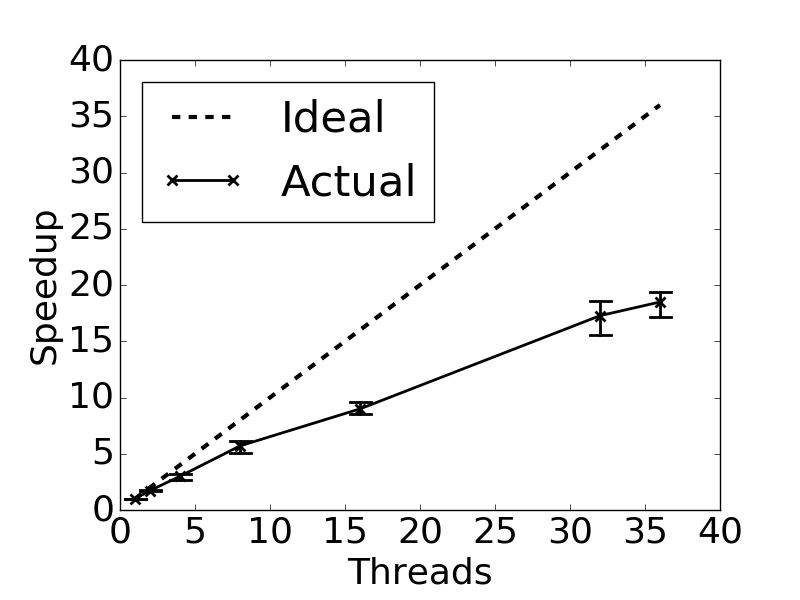
\includegraphics[width=\linewidth]{figures/fs-parallel-scaling-tracks.png}
		\caption{By Tracks}
		\label{fig:rt-parallel-fs-tracks}
	\end{subfigure}
	\begin{subfigure}{0.45\textwidth}
		\centering
		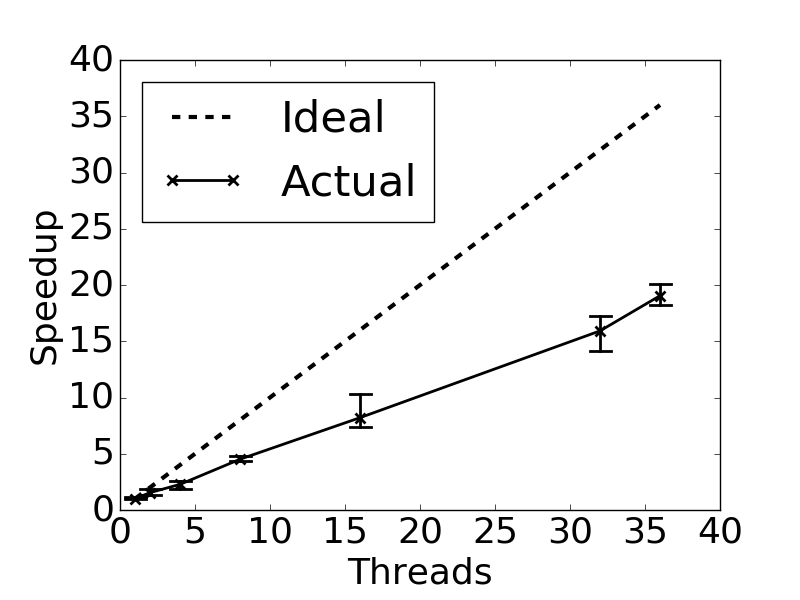
\includegraphics[width=\linewidth]{figures/fs-parallel-scaling-stacks.png}
		\caption{By $Z$-Stacks}
		\label{fig:rt-parallel-fs-stacks}
	\end{subfigure}
	\caption[]{Strong scaling of the SDSA test problem on the Falcon supercomputer using on-the-fly ray tracing by (a) tracks and (b) $z$-stacks.}
	\label{fig:rt-parallel-fs}
\end{figure}


NOTE THE FULL THREAD RESULTS FOR FALCON AND CETUS

	method --	machine -- number of threads -- time
tracks
stacks



%------------------------------------------------------------------------------
%
%------------------------------------------------------------------------------
\section{CONCLUSION} 

In this study, an alternative approaches to 3D \ac{MOC} were presented for segment storage whereby only 2D segments are stored and 3D segments are computed on-the-fly. This approach offers significant memory reduction with minimal or no computational overhead. Results show that the most efficient ray tracing tested was ray tracing entire $z$-stacks of 3D tracks with temporary storage of the computed segments.
\clearpage

\vfill
\begin{highlightsbox}[frametitle=Highlights]
\begin{itemize}
  \item The bias between OpenMC and OpenMOC is the result of the flux separability approximation which uses the scalar rather than the angular flux to collapse the total \ac{MGXS} in energy and space.
  \item The most rigorous solution would require the use of angular-dependent total \ac{MGXS}. However, most deterministic multi-group methods, including OpenMOC, are not equipped to use angular-dependent \ac{MGXS}.
  \item \ac{SPH} factors are introduced here as one approach to force reaction rate preservation in multi-group methods which use \ac{MC}-generated \ac{MGXS}.
  \item The \ac{SPH} factor scheme corrects the total \ac{MGXS} to enforce neutron balance with a reference fixed source computed from \ac{MC} tallies.
  \item The flux errors and eigenvalue bias between OpenMC and OpenMOC was largely resolved with \ac{SPH} factors for a 1D slab and 2D fuel pin.
  \item It is unclear if a generalizable scheme based upon \ac{SPH} factors may be used to correct for the flux separability approximation.
  \item Future work should investigate methods to account for the angular dependence of total \ac{MGXS} in order to adequately preserve reaction rates in fine-mesh transport methods with \ac{MC}-generated \ac{MGXS}.
\end{itemize}
\end{highlightsbox}
\vfill